% Definition of circles
\def\firstcircle{(0,0) circle (1.5cm)}
\def\secondcircle{(0:2cm) circle (1.5cm)}
\def\thirdcircle{(1,-1.5) circle (1.5cm)}

\colorlet{circle edge}{blue!50}
\colorlet{circle area}{blue!20}

\tikzset{filled/.style={fill=circle area, draw=circle edge, thick},
    outline/.style={draw=circle edge, thick}}

\setlength{\parskip}{5mm}

%--
\begin{enumerate}

\item a) \\
% Set A but not B
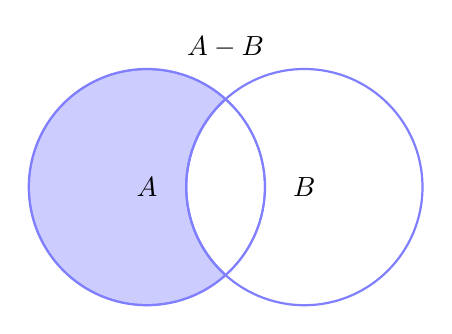
\begin{tikzpicture}
    \begin{scope}
        \clip \firstcircle;
        \draw[filled, even odd rule] \firstcircle node {$A$}
                                     \secondcircle;
    \end{scope}
    \draw[outline] \firstcircle
                   \secondcircle node {$B$};
    \node[anchor=south] at (current bounding box.north) {$A - B$};
\end{tikzpicture}

\item b) \\
%Set A or B but not (A and B) also known a A xor B
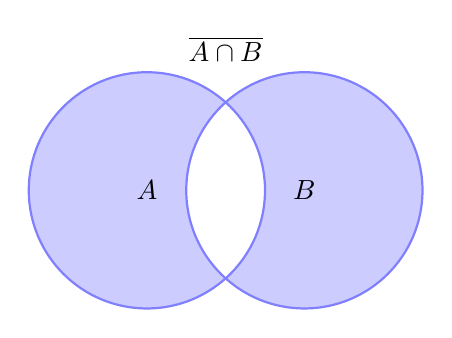
\begin{tikzpicture}
    \draw[filled, even odd rule] \firstcircle node {$A$}
                                 \secondcircle node{$B$};
    \node[anchor=south] at (current bounding box.north) {$\overline{A \cap B}$};
\end{tikzpicture}

\item c) \\
% Set A and B and C
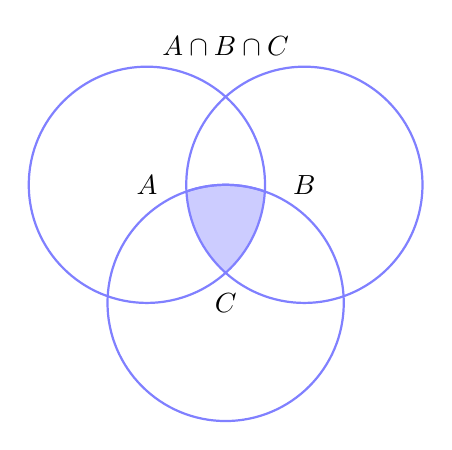
\begin{tikzpicture}
    \begin{scope}
        \clip \firstcircle;
	\clip \secondcircle;
        \fill[filled] \thirdcircle;
    \end{scope}
    \draw[outline] \firstcircle node {$A$};
    \draw[outline] \secondcircle node {$B$};
    \draw[outline] \thirdcircle node {$C$};
    \node[anchor=south] at (current bounding box.north) {$A \cap B \cap C$};
\end{tikzpicture}

\item d) In diesem Fall stellt weiß die markierung da! \\
%Set A or B but not (A and B) also known a A xor B
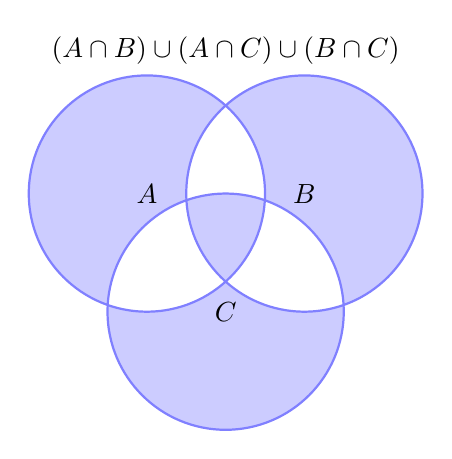
\begin{tikzpicture}
    \draw[filled, even odd rule] \firstcircle node {$A$}
                                 \secondcircle node{$B$}
				 \thirdcircle node {$C$};
    \node[anchor=south] at (current bounding box.north) {$(A \cap B) \cup (A \cap C) \cup (B \cap C)$};
\end{tikzpicture}



\end{enumerate}

